\documentclass[10pt, a4paper]{article}
\usepackage[margin=0.7in]{geometry}
\usepackage{fancyhdr}
\usepackage{graphicx, caption}
\graphicspath{ {images/} }
\pagestyle{fancy}
\lhead{Hot or Cold}
\chead{Mobile Application Development}
\rhead{Group 1}
\fancyfoot{}
\cfoot{Page \pagename}	
\setlength{\headheight}{25pt}
\renewcommand{\headrulewidth}{0.4pt}
\renewcommand{\footrulewidth}{0.4pt}
\begin{document}

\title{Hot or Cold - 15COB155 Coursework 2}
\author{Team 1 | Mobile Application Development}
\maketitle
\begin{center}
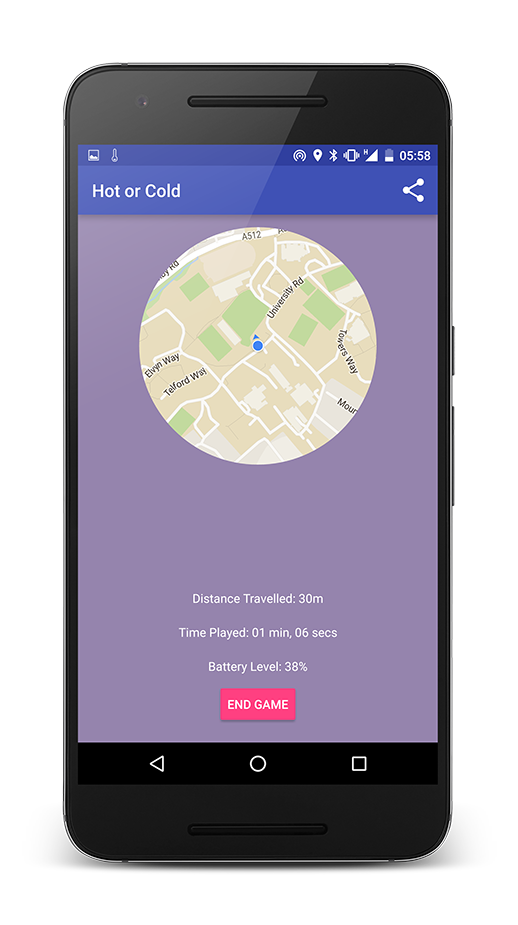
\includegraphics[height=0.82\textheight]{phone_game_2}
\end{center}
\newpage

\section*{Specification}
\begin{itemize}
\item The user will see a splash screen on startup
\begin{itemize}
\item The splash screen will show until the app has finished loading in the background
\item The splash screen will redirect to the home screen once the app has finished loading
\item The splash screen will only show the first time the app is loaded from memory
\end{itemize}

\item The app will check whether the user has enabled GPS
  \begin{itemize}
  \item If the user has GPS disabled then:
  \begin{itemize}
    \item A notification will appear informing the user that GPS is required
    \item The notification will be able to be clicked and will take the user to their GPS settings
    \item The notification will appear indefinitely
    \item If the user turns on GPS and goes back to the app then a notification will appear indicating that the GPS has been turned on
  \end{itemize}
\end{itemize}

\item The user will be able to see a leaderboard
	\begin{itemize}
		\item The leaderboard will show a list of scores in descending order
        \item The leaderboard will be stored locally in a SQLite database
	\end{itemize}

\item The user will be able to start a new game
	\begin{itemize}
		\item The user will be able to setup a maximum distance for the game
        \item Once the user starts the game the app will select a random location within that distance that the user will have to try and locate
	\end{itemize}
    
\item The user will be able to double tap the home screen to start a quick game

\item The user will be able to earn points for getting to the goal
	\begin{itemize}
		\item Less points will be earned if they set a lower maximum distance
        \item More points will be earned if they  set a higher maximum distance
        \item Less points will be earned if they finish further away from the goal
        \item More points will be earned if they finish closer to the goal
	\end{itemize}

\item When the user starts a game there will be a screen that shows them how close they are to the hotspot by colour
	\begin{itemize}
		\item The background will get more red the closer the player is to the goal
        \item There will be a map on the screen which will show the user their current location
        \item The user will be able to press a button which allows them to end the game
        \item The user will be able to see how far they have traveled while playing the game
        \item The user will be able to see how long they have been playing the game
        \item The user will be able to see their battery percentage on the in game screen
	\end{itemize}


\item When the user ends the game they are taken to a game complete screen
	\begin{itemize}
		\item The screen will tell the user how many points they scored for that game
        \item The user will be able to open the location of the hotspot in google maps
        \item The user will be able go to the leaderboard screen by pressing a button
        \item The user will be able press a button to take them to the home screen
	\end{itemize}

\item When in an active game there will be a notification in the notification bar
\begin{itemize}
\item The notification will be destroyed when the user ends the game
\end{itemize}

\item The user will be able to rotate the screen throughout the application

\item The user will be able to view more ‘fragments’ on a larger device
\begin{itemize}
\item The home screen will always be shown on the left hand side of the screen
\item The current screen will be shown on the right hand side of the screen
\end{itemize}

\end{itemize}


\section*{Application Overview}
\paragraph{•}
Our mobile application is a game called `HotOrCold'. For users to play the game, the application generates a geo `hotspot' which users then have to go out and find. Users can give up at any time and `cash in' the points they've gained by getting close to the hotspot, but there is an incentive to keep on trying to get as close as possible because the number of points earned increases exponentially as the users get closer to the target. The challenge in this game is that the users do not know the geographic co-ordinates of the geo hotspot, they only know if they are getting closer (hotter) or further away (colder) through the application's `temperature gauge'.

\paragraph*{•}
Users are also able to set the difficulty of the game by choosing the maximum distance from their current location that the hotspot can be generated. Hotspots that are generated on a higher difficulty level (i.e. at a further distance from the user's starting location) then enable the user to gain more points for getting close to the target than if they had selected a shorter distance.

\paragraph*{•}
Whilst users are in the application they can share that they are using the application with friends at any time by clicking the `Share' button on any of the application screen. In addition to this, the game has a  notification in the notification bar when the user is in game that enables the application to continue running in the background, even whilst the app is not open.

\paragraph*{•}
Upon completing a game or giving up, users are presented with a `Game Complete' screen: this will display the score that they achieved for that game and will reveal the true location of the hotspot that the game had used through a button that will open the location of the expired hotspot in Google Maps. In the background this will also use a content provider to add the latest score to a list in local storage which is used to populate the leaderboard screen. The leaderboard screen shows a list of scores of the games that have been played in order from highest to lowest.

\section*{Software Structure Overview}
\paragraph{•}
When the app is first loaded the user is shown a splash screen while the app loads in the background. After the app is loaded they will be taken to the home screen via an explicit intent. On the home screen they are able to press two different buttons which will either take them to the leaderboard or to the start game screen. If they go to the leaderboard screen they will be able to see all the games that have been played on that device and their scores in descending order, they also will be able to press the back button to go back to the home screen. If the user chooses to go to the start game screen they will be shown a slider that allows them to choose the the maximum distance for the game and a button which starts the game and takes the user to the in game screen, the user can also press the back button to go back to the home screen. When on the in game screen the user is shown a map, the center of which is the user's current location, some text which indicates the distance that the user has traveled, how long the user has been playing for and the devices' battery percentage. A button allows the player to end the game. While on this screen, the user can move about and the background of the in game screen will change to be more red the closer they get to the randomly generated `hotspot'. When the user thinks that they've reached the hotspot, or wishes to give up, they can press the button labeled `end game' which will take them to the game complete screen where they are able to view the score they achieved for their guess at the hotspot, a button which will take them to the leaderboard and a button which will take them to the home screen.

*Insert flow diagram here*

\paragraph*{•}
We decided to develop the application in two parts, the first part being the application itself, and the second part being an API that handled most of the game logic. The application section includes all of the code that deals with android functions and all of the UI code, whilst the API deals with starting games, keeping game scores, calculating distances to the locations and the respective color for the screen based on that distance.

\paragraph*{•}
The application starts on the `Splash Activity' which displays an image while the app is loading. Once the app has loaded, an explicit intent is used to get to the `Main Activity' which is used for the rest of the app. On load the `Main Activity' will start the Location Service which performs functions such as checking to see whether the GPS is disabled using the onProviderDisabled function. If GPS is disabled a snackbar is shown which the user can then click to got to the GPS settings using an implicit intent. The user can then enable the GPS and press the back button to return to the app. Upon the users return they will be shown a snackbar thanking them for enabling the GPS. The `Main Activity' inflates the the `home fragment' so as to display our main home screen and provide the user with options to navigate futher into our application. When the `Main Activity' is created, a static instance of the GameManager object is created. This is where the app calls all the API functions to deal with various parts of the game's functioning.

\paragraph*{•}
Because our app uses mostly fragments we had to manually handle the backstack to allow the user to use the back button to navigate backwards through the fragments that they used. To do this we had to manually add the fragment to the backstack. In some cases in our app though we didn't want to allow the user to go back to the previous fragment, for instance after the user has completed the game we didn't want to allow the user to go back to the game screen and continue playing. To allow this we changed the functionality of the android back button on the `end game fragment' to take the user to the `home fragment'. Our app uses two layouts for the fragments, on a smaller device only the current fragment is displayed. Whereas on a large screen two fragments are displayed, the `home fragment' on the left hand side of the screen and the current fragment is displayed on the right hand side.

\paragraph*{•}
When the `home fragment' is inflated, two buttons are displayed which each link to a different fragment: the `leaderboard fragment' and the `start game fragment'. Users can also double tap on the home screen to quickly start a game that generates a random hotspot within 10 kilometers of the user. When the `leaderboard fragment' is inflated a ListView is created which is filled with data using a cursor and adapter. The cursor get's filled with data by querying the custom content provider MyScoreProvider for all rows in the database, which it then sorts by the ``SCORE\_VALUE'' column in descending order. The cursor is then added to a SimpleCursorAdapter which uses the data in the cursor to load the score value and the score time. The cursor adapter is then added to the list view where it is used to populate the list.

\paragraph*{•}
Our app is a location based app, and therefore we need to continually keep the location up-to-date. In order to do this, we have the main activity implementing the LocationListener class. We activate the location listener and have it callback to our class whenever the location is updated. We then store this location in a private static variable, which is updated continually as the location changes. When a game is started, it updates the interface once every second by grabbing the location from the variable in the MainActivity. During each update, it calls the game API, providing the new location so that it can be stored for later use as well as getting the new color for the screen.

\paragraph*{•}
The `start game fragment' contains a SeekBar which is used to select the maximum radius for the hotspot to be created in and a Start Game button which when clicked will attempt to start a game. This fragment uses the Location Service in order to get the current location for use when starting the game. If the phone has been unable to connect to the GPS by this point, the current location will be returned as null and so it will cause the phone to vibrate and produce a snackbar, informing the user that it is still searching for GPS signal and therefore will not start the game. If the fragment was successful in getting a location it will start a new game in the GameManager object, passing the current location and the progress of the Seekbar, to make a new Game object in the GameManager which then starts managing various parts of the game.  After creating the new Game through the GameManager, the `in game fragment' is inflated to begin the game. When the device is rotated the value of the SeekBar needs to be retained, to do this we have to save the value in the instance state, and when the fragment loads we have to check if the value is set and if it is use the value to populate the SeekBar's progress.

\paragraph*{•}
On creation of the `in game fragment' a notification is created in the notification bar, this notification informs the user that a game is in progress. A text view is shown, this displays the total distance traveled so far and another text view shows the elapsed game time. A third text view shows the battery percentage level, this is implemented using a BroadcastReceiver, when an ``ACTION\_BATTERY\_CHANGED'' event is received it get's the current battery level and updates the text view. There is also circular map in the center which displays the user's current location, this is implemented by drawing the map and then drawing a bitmap the same colour as the background on top of it with a circular hole cut into it. On creation of the map it zooms in from the default camera zoom to a much closer one and adds a location listener which updates the colors of both the background of the fragment and of the circle around the map. It also updates the position of the center of the map to be the updated location as well as updating the distance traveled text view and the Time played text view by using calls to the API. The API is informed of the new location when it is called to work out the updated colour of the backgrounds. At the bottom of the fragment there is a button which when pressed signals to the Game in the GameManager that the game has ended, destroys the game in progress notification and inflates the `game completed fragment'. Like the `start game fragment', the `in game fragment' also needs to store some information in a Bundle to handle activity lifecycle events such as screen rotation. In this case we have to store the latitude and longitude for the map so that when we create the map again it will keep the centering and the blue dot for the user's location.

\paragraph*{•}
The `game complete fragment' uses a custom view called a `KeyValueView' which is a custom view for displaying some data and a label next to each other. It is used to display the score that the user gained in their game which is returned by a call to the API using the previous game. The fragment also has two buttons, one which inflates the `leaderboard fragment' and the other, which only appears only on smaller devices, inflates the `home screen'.

\section*{Application Functionality}

\paragraph*{•}
We implemented a splash screen by using an activity which displays a mipmap image and then intents to the Main Activity. This means that the splash screen will wait until the Main Activity has fully loaded.

\paragraph*{•}
The app checks whether the GPS has been enabled by creating a LocationManager, then if the provider is disabled the onProviderDisabled function will show a snackbar indefinitely with text ``Please switch on GPS'' which contains an option that can be clicked to take the user to the GPS settings. If the provider is enabled after being detected as disabled a snackbar with text ``GPS is On - Thank You'' is shown briefly.
\paragraph*{•}
We have implemented a leaderboard screen, this uses a custom Provider called `MyScoreProvider' which loads scores that have been stored in a sqlite database (local storage). When loading the data into the cursor the data from the database is sorted into descending order.

\paragraph*{•}
Our app has a start game screen, on it is a slider that enables the user to modify a distance within which the app will randomly generate a hotspot.

\paragraph*{•}
If the user double taps on the home screen, a new game will be created with an objective within 10 kilometers of the users location and the user will be taken to the in game screen.

\paragraph*{•}
The amount of points awarded to the user is defined as follows, where x = the current distance from the hotspot and y = the number of points scored:
\[y = 0.1((x-50) + (0.2x)^2\]
When plotted this graph gives the user gets no points when they have traveled less than 50 meters, as we don't count negative scores, and when the user travels further they gain more points. The user will only ever be able travel as far as the hotspot, so if the hotspot is generated closer they will gain less points than if it was generated further away.

\paragraph*{•}
The background colour of the in game screen is calculated using the calculateDistanceColour function in the Game object in the API, it does this by calculating the percentage distance between the user's current distance from the hotspot and the distance they started at using simply:
\[percentage = (startDistance - currentDistance)/startDistance\]
If this is less than zero then the percentage is capped at 0 and the the currentDistance is set as the new startDistance, we then work out the colour that percentage between the blue and red that we picked as our maximum and minimum. We do this by calculating the value for each colour and then combining them into a hex string.
By using this calculation when the user get's further away from the hotspot than they started the most blue blue will be show, and any time the user get's closer to the hotspot, even if they are currently further away from the hotspot than they started the screen will always get more red as the user get's closer to the hotspot.

\paragraph*{•}
The in game screen shows a map with a Google Map LocationChangeListener attached which updates so that the user's position is always in the center of it, with a blue dot as an indicator for the user's position. This LocationChangeListener also pans the map `camera' to ensure that the animation in between the user's registered co-ordinates is smooth. We also make a call to the Game Manager's getHeatHex method, to calculate the new hexadecimal colour code for the background of the in game screen, and then apply it as the new background colour every time the user's location changes.

\paragraph*{•}
The in game screen also shows three text views which indicate the distance traveled so far, the total time playing and the devices current battery percentage. The distance traveled is returned by the getTravelDistance function on the Game object which iterates over the list of stored location working out the distance between each location. When the game is started a datetime is stored and compared to whenever the text is updated.

\paragraph*{•}
A share option is available in all screens of the application, this is provided by a ShareActionProvider that creates a menu of sharing options for the user to choose from. If the user then chooses an option they can send a message to a friend informing them that they are using the HotOrCold application.

\paragraph*{•}
There is also a button labeled ``End game'' which allows the user to end the game, this signals to the Game Manager that the game has ended using the endCurrentGame function. The Game Manager then set's the current game as the previous game and signals the the game that it has ended.

\paragraph*{•}
The ``End game'' button on the in game screen redirects the user to the game complete screen. This screen has a custom KeyValue view which it uses to display the points that the user gained for playing the game. It also displays three buttons which allow the user to navigate to the leaderboard, home screen or to open the location of the hotspot in Google Maps by getting the location from the previous game object's objective from which the latitude and longitude is used in an implicit intent which loads a list of application with which the user can select an app that will take the data. The ending games' score is also saved to the SQLite database at this point.

\paragraph*{•}
When the in game screen is loaded it also builds and loads a notification for the app. When the game is ended, if the notification is still in the notification bar, the notification is destroyed.

\paragraph*{•}
The user will be able to rotate their device at any point whilst using the app and the layout will update accordingly. This is possible because we have worked with the activity lifecycle to ensure that any user data is stored, and then re-loaded into the view when it is destroyed and re-created as the layout switches to the other orientation.

\paragraph*{•}
On a larger screen size such as a Tablet the Activity is designed to be able to display two fragments side-by-side, the left side fragment always display the home screen, the right sided fragment content changes depending on which fragment is being inflated. We implemented different layouts for portrait and landscape orientations so as to fully utilise the space available on the device.

\newpage

\section*{Technical Requirements}
Discussion and justification of which technical requirements were met / not met
\\
\linebreak
\begin{tabular}{|p{0.2\textwidth} | p{0.75\textwidth}|}
\hline 
Requirement & A minimum of three distinct screens \\ 
\hline 
Mandatory / Optional & Mandatory \\ 
\hline 
Completed & Yes \\ 
\hline 
Evidence & Our application has 5 distinct screens, a Home Screen, Start Game Screen, In Game Screen, End Game Screen and a Leaderboard Screen. \\ 
\hline 
\end{tabular} 
\\
\linebreak
\linebreak
\begin{tabular}{|p{0.2\textwidth} | p{0.75\textwidth}|}
\hline 
Requirement & Work properly with the app lifecycle (include rotate screen changes) \\ 
\hline 
Mandatory / Optional & Mandatory \\ 
\hline 
Completed & Yes \\ 
\hline 
Evidence & In the start game and in the in game fragment we use a saved instance state to store information that needs to be kept when the device is rotated. For example in the start game fragment there is a slider for which we need to store the value of, when the fragment is deleted we store the value in the saved instance state bundle and when the fragment is created, we check to see if the value has been set in the bundle and if it has set it to the stored value. \\ 
\hline 
\end{tabular} 
\\
\linebreak
\linebreak
\begin{tabular}{|p{0.2\textwidth} | p{0.75\textwidth}|}
\hline 
Requirement & Use permissions and use them responsibly \\ 
\hline 
Mandatory / Optional & Mandatory \\ 
\hline 
Completed & Yes \\ 
\hline 
Evidence & We use Fine and Course Locations so that we can get the users location.  We require the Vibrate permission to produce a vibrate when the still searching for GPS snackbar is produced, this vibrate helps to alert the user that the game has not been started yet. The Internet permission is used to produce the Map view on the In Game Screen.  \\ 
\hline 
\end{tabular} 
\\
\linebreak
\linebreak
\begin{tabular}{|p{0.2\textwidth} | p{0.75\textwidth}|}
\hline 
Requirement & Use intents to move inside your app and to an outside app \\ 
\hline 
Mandatory / Optional & Mandatory \\ 
\hline 
Completed & Yes \\ 
\hline 
Evidence & When the app is first loaded into memory we use an explicit intent to move from the Splash Activity to the Main Activity. We also use implicit intents throughout the app, one implicit intent is used when we reveal give the user the options to reveal the final hotspot location from the end game screen.  To accomplish this we send the hotspot latitude and longitude to any application that accepts a ACTION\_VIEW Intent.\\ 
\hline 
\end{tabular} 
\\
\linebreak
\linebreak
\begin{tabular}{|p{0.2\textwidth} | p{0.75\textwidth}|}
\hline 
Requirement & Create and use your own ContentProvider \\ 
\hline 
Mandatory / Optional & Mandatory \\ 
\hline 
Completed & Yes \\ 
\hline 
Evidence & The MyScoreProvider deals with saving data to and loading data from the SQLite local storage and provides the ability to send the queries to the ScoreDBHelper which uses the ScoreDataModel as the reference for table and field names \\ 
\hline 
\end{tabular} 
\\
\linebreak
\linebreak
\begin{tabular}{|p{0.2\textwidth} | p{0.75\textwidth}|}
\hline 
Requirement & Create and use your own Custom Loader \\ 
\hline 
Mandatory / Optional & Mandatory \\ 
\hline 
Completed & Yes \\ 
\hline 
Evidence & On the leaderboard screen we use a SimpleCursorAdapter to load our scores in descending order from our custom data provider. \\ 
\hline 
\end{tabular}
\\
\linebreak
\linebreak
\begin{tabular}{|p{0.2\textwidth} | p{0.75\textwidth}|}
\hline 
Requirement & Make use of local storage \\ 
\hline 
Mandatory / Optional & Mandatory \\ 
\hline 
Completed & Yes \\ 
\hline 
Evidence & We utilise an SQLite database for storing the final score from each game for persistence between games and to fill the Leaderboard \\ 
\hline 
\end{tabular} 
\\
\linebreak
\linebreak
\begin{tabular}{|p{0.2\textwidth} | p{0.75\textwidth}|}
\hline 
Requirement & Use a different UI for tablets \\ 
\hline 
Mandatory / Optional & Mandatory \\ 
\hline 
Completed & Yes \\ 
\hline 
Evidence & The UI on tablets uses a dual view which has the `home screen fragment' on the left, and then the various other views such as the `game screen fragment', `leaderboard fragment' and `game complete fragment \\ 
\hline 
\end{tabular} 
\\
\linebreak
\linebreak
\begin{tabular}{|p{0.2\textwidth} | p{0.75\textwidth}|}
\hline 
Requirement & Receive Broadcast events and make use of them in meaningful ways \\ 
\hline 
Mandatory / Optional & Optional \\ 
\hline 
Completed & Yes \\ 
\hline 
Evidence & We receive the broadcast events to notify the user about their battery level changing and if their battery level gets too low (ie 15\%). We received these broadcast events as our application uses GPS to track the user, this can be a significant drain to the phones battery, therefore we want to warn the user when their battery level gets low so that they consider closing the app.\\ 
\hline 
\end{tabular} 
\\
\linebreak
\linebreak
\begin{tabular}{|p{0.2\textwidth} | p{0.75\textwidth}|}
\hline 
Requirement & Create and use a custom view \\ 
\hline 
Mandatory / Optional & Optional \\ 
\hline 
Completed & Yes \\ 
\hline 
Evidence & We have created a Custom View called KeyValueView this is used on the Game Completed page to display to the user the points that they gained in the game. \\ 
\hline 
\end{tabular} 
\\
\linebreak
\linebreak
\begin{tabular}{|p{0.2\textwidth} | p{0.75\textwidth}|}
\hline 
Requirement & Implement ShareActionProvider \\ 
\hline 
Mandatory / Optional & Optional \\ 
\hline 
Completed & Yes \\ 
\hline 
Evidence &  We implemented a ShareActionProvider in the Main Activity to allow users to share how much they love the HotOrCold application with any available sharing option.\\ 
\hline 
\end{tabular} 
\\
\linebreak
\linebreak
\begin{tabular}{|p{0.2\textwidth} | p{0.75\textwidth}|}
\hline 
Requirement & Use Services \\ 
\hline 
Mandatory / Optional & Optional \\ 
\hline 
Completed & Yes \\ 
\hline 
Evidence & In the MainActivity we initialise and start the LocationService which manages getting and storing the most recent location from the GPS in the device \\ 
\hline 
\end{tabular} 
\\
\linebreak
\linebreak
\begin{tabular}{|p{0.2\textwidth} | p{0.75\textwidth}|}
\hline 
Requirement & Use Notifications \\ 
\hline 
Mandatory / Optional & Optional \\ 
\hline 
Completed & Yes \\ 
\hline 
Evidence & When the InGameFragment is started, it creates a notification which is added to the notification bar. This notification is deleted once the game ends \\ 
\hline 
\end{tabular} 
\\
\linebreak
\linebreak
\begin{tabular}{| p{0.2\textwidth} | p{0.75\textwidth} |}
\hline 
Requirement & Capture touch gestures \& make reasonable use of them \\ 
\hline 
Mandatory / Optional & Optional \\ 
\hline 
Completed & Yes \\ 
\hline 
Evidence & In the HomeScreenFragment class we add a touch listener which listens for a double tap which starts a new game at a random distance \\ 
\hline 
\end{tabular} 
\\
\section*{Testing}
\paragraph*{•}
\begin{tabular}{| p{0.22\textwidth} | p{0.22\textwidth} | p{0.22\textwidth} | p{0.22\textwidth} |}
\hline 
\textbf{Feature}
& \textbf{Test Case}
& \textbf{Expected Result}
& \textbf{Actual Result} \\ 
\hline 
The user will be able to navigate to a leaderboard screen
& Open the home screen and press the button labeled ``Leaderboard''
& The leaderboard is shown
& Once the leaderboard is shown the screen shown in fig. 4 was shown. \\ 
\hline 
The user will be able to see top scores of games they've played
& Open the leaderboard screen after playing a few games
& The scores from the played games will be shown in descending order on the leaderboard
& As shown in fig. 4, the scores are displayed in descending order \\ 
\hline 
The user will be able to see their latest scores in the leaderboard
& Open the leaderboard after playing at least one game
& The user's score appears on the leaderboard
& After playing a game (fig. 9), the score appears on the leaderboard in fig. 4 \\ 
\hline 
The user will be able to get to the game setup screen
& Open the home screen and press the button labeled ``Start Game''
& The game setup screen is shown
& Once the button labeled ``Start game'' was pressed (fig. 5), the start game screen appeared fig. 12 \\ 
\hline 
The user will be able to start the game
& Open the game setup screen and press the button labeled ``Start Game''
& The game screen is shown
& Once the button labeled ``Start game'' was pressed (fig. 11), the game screen appeared fig. 1 \\ 
\hline 
The user will be able to change the maximum distance for the ``hotspot''
& Open the game setup screen and use the slider
& The user will be able to move the slider and the distance shown will change
& Once we moved the slider from fig. 11 to fig. 12 the distance displayed changed \\ 
\hline 
The user will be able to change the maximum distance for the ``hotspot''
& Open the game setup screen, move the slider to a far away distance and press the start the game
& When the user moves to try and locate the ``hotspot'' the screen's colour might change less than quickly than if the distance was set to closer
& When we tested this with the distance set to high and the distance set to low, the app with the distance set to low change much quicker than the app with the distance set to high \\ 
\hline
The game screen will change from a blue to a red as the user get's closer to the ``hotspot''
& Start a new game and when the user moves the colour will get more red only when moving in one direction
& The colour will only get more red when moving in one direction
& When moving in one direction the background stayed the same blue (fig. 1) but once we moved in the other direction the background started to get more red (fig.3) \\ 
\hline 
There will be a notification in the notification bar while the game is playing
& Start a new game and check the notification bar for a notification
& There will be a notification for the app in the notification bar
& After starting the game a notification appeared in the notification bar as in fig. 7 \\ 
\hline 
The notification will persist when the application is closed
& Start a new game and then close the app, then check the notification bar for a notification
& There will be a notification for the app in the notification bar
& On closing of the app, the notification persists as in fig. 7 \\ 
\hline 
The notification will close when the game is finished
& Start a new game and then end the game, then check the notification bar for a notification
& There will not be a notification for the app in the notification bar
& Once the game is finished the notification disappears as in fig. 9 \\ 
\hline 
\end{tabular} 

\begin{tabular}{| p{0.22\textwidth} | p{0.22\textwidth} | p{0.22\textwidth} | p{0.22\textwidth} |}
\hline 
\textbf{Feature}
& \textbf{Test Case}
& \textbf{Expected Result}
& \textbf{Actual Result} \\ 
\hline 
While playing the game, the user will be able to end the game
& Start a new game and press the ``End Game'' button
& The user is taken to the game complete screen
& Once the ``End Game'' was pressed the we were taken to the game complete screen shown in fig. 9 \\ 
\hline 
While playing the game, the user will be able to see their current location in the middle of the screen
& Start a new game
& There is a circle filled with a map in the middle of the screen, the center of the map is the current location
& On opening the game screen there is a circular map in the middle top of the screen as shown in fig. 1 \\ 
\hline 
While in the app, the user will be able to press a button to share their love for the app
& Press the ``Share'' button in the top bar
& The user will be able to share the message to an option in the share menu
& Clicking the share button produces a list of options to share the message by (fig. 16)  \\ 
\hline
While playing the game, the user will be able to see how far they have traveled so far
& Start a new game
& After the user has moved about a bit they will be able to see how far they have traveled so far
& The distance travelled is visible on the in game screen (fig. 1)  \\ 
\hline
On the end game screen the user will be able to open Google Maps to show the final location
& Start a new game, press the ``End Game'' button, press the button labeled ``Show final destination''
& The app will open up Google Maps and show the final destination
& Clicking on the ``Reveal Location'' button loads the location of the final destination in Google Maps \& Clicking on the ``Reveal Location'' button loads the location of the final destination in Google Maps (fig. 6)\\ 
\\ 
\hline
On the end game screen the user will be able to see the points that they got for their guess
& Start a new game, press the ``End Game'' button
& The user will be able to see the points that they gained for that Game
& The points total is displayed on the end game screen (fig. 9) \\ 
\hline
\end{tabular} 

\section*{Conclusion}
\paragraph*{•}
While we were able to include a wide variety of features, there where a few features that we wished that we could have implemented. We originally planned to have an instruction screen that would give users a walkthrough on how to use the app, users would have been able to swipe through several screens using touch gestures. However, due to time constraints we were unable to complete this in time so it was scrapped. If we had been able to complete the feature we could have implemented it as a fragment containing cards or perhaps a list view filled with text and/or images that would have explained to the user how to use our app, we would have had to also given some indication that the have to scroll through the instructions so we would have put some text in to explain this. We also planned to give the user the ability to edit preferences within the app for example they would have been able to set a unit preference. If you look in the code of the API and a few of the fragments involving distances you might see that we have included a few functions ready for when the feature was implemented. We would have had a separate activity that would allow us to change the preferences with a preferences object that could be saved in local storage and queried by various parts of the app when settings are needed. We also would have had a more feature full notification that wouldn't allow the user to swipe it away and would give the user some indication of their progress in the game.
\paragraph*{}
Other than the three features mentioned above we believe we have a very functionaly high-quality application that meets all of the requirements. The application works exactly as intended, allowing the user to explore an area by setting a random location for them to find. We have incorporated different layouts for a variety of devices and can therefore cater to a larger market.

\newpage

\section*{Figures}

\begin{figure}[!htb]
\minipage{0.32\textwidth}
  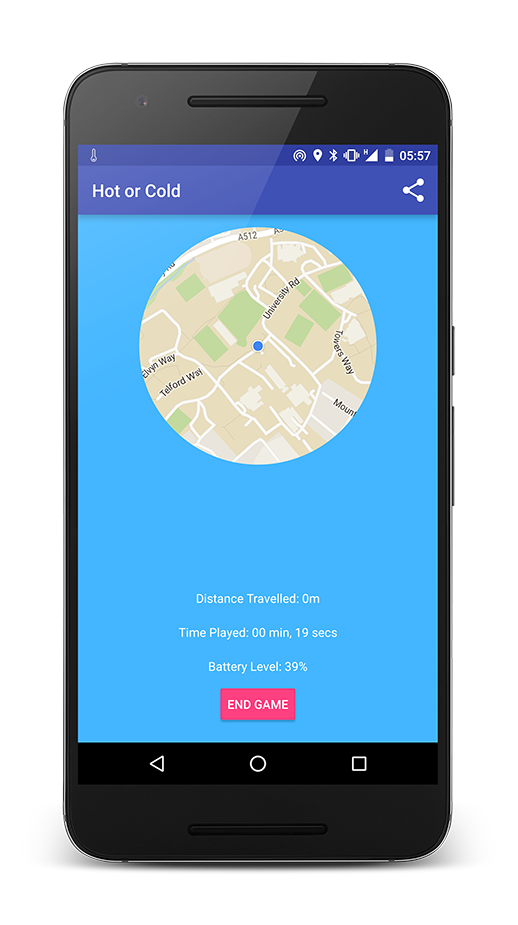
\includegraphics[width=1.0\textwidth]{phone_game_1}
  \caption{}
\endminipage\hfill
\minipage{0.32\textwidth}
  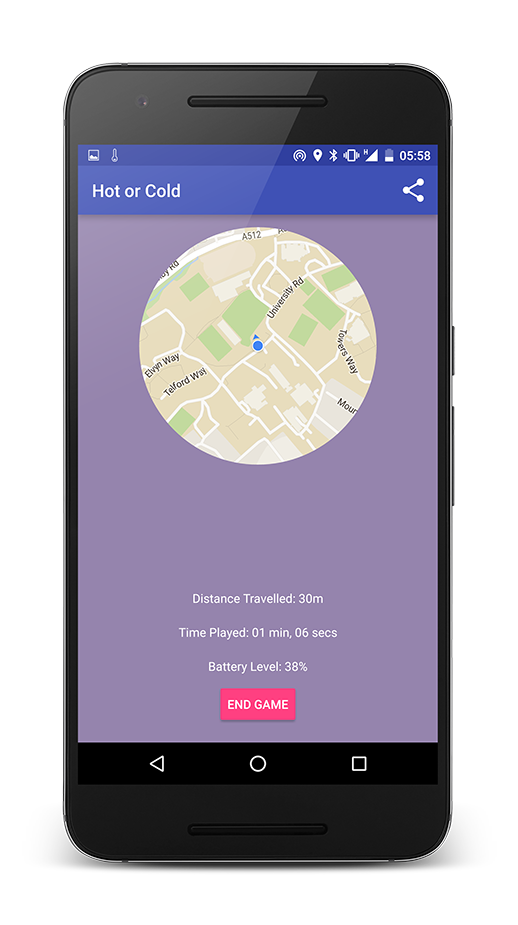
\includegraphics[width=1.0\textwidth]{phone_game_2}
  \caption{}
\endminipage\hfill
\minipage{0.32\textwidth}%
  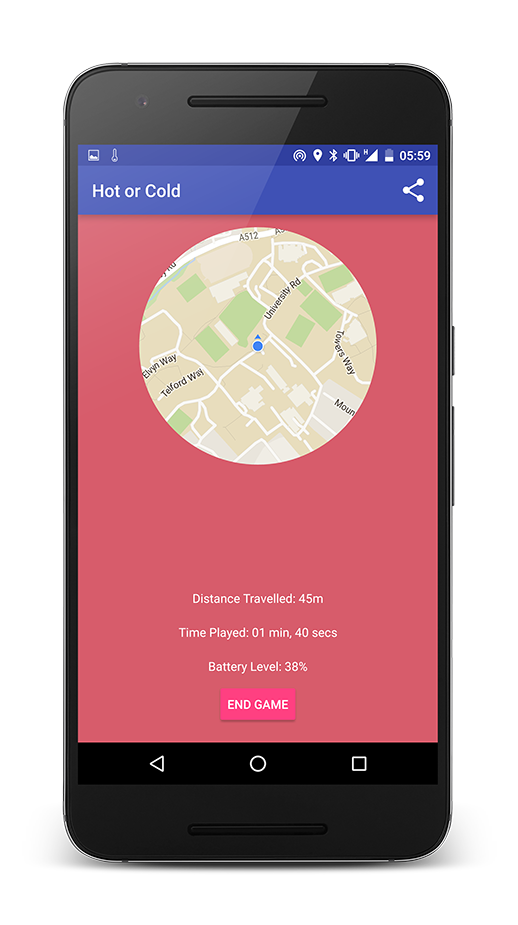
\includegraphics[width=1.0\textwidth]{phone_game_3}
  \caption{}
\endminipage
\end{figure}

\begin{figure}[!htb]
\minipage{0.32\textwidth}
  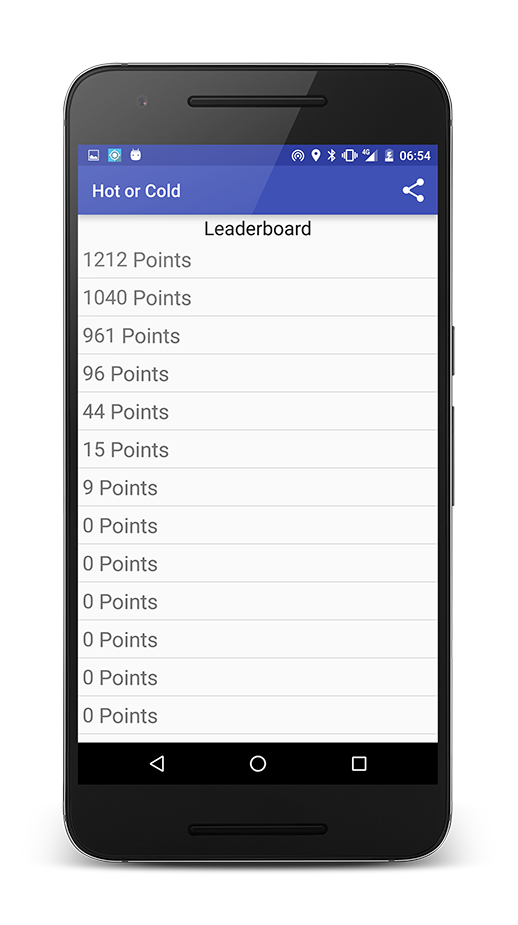
\includegraphics[width=1.0\textwidth]{phone_leaderboard_1}
  \caption{}
\endminipage\hfill
\minipage{0.32\textwidth}
  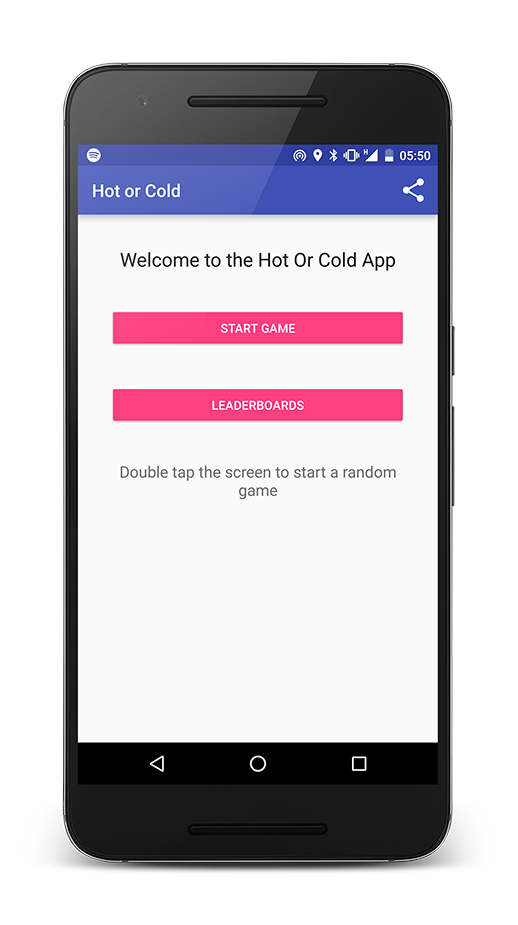
\includegraphics[width=1.0\textwidth]{phone_mainscreen_1}
  \caption{}
\endminipage\hfill
\minipage{0.32\textwidth}%
  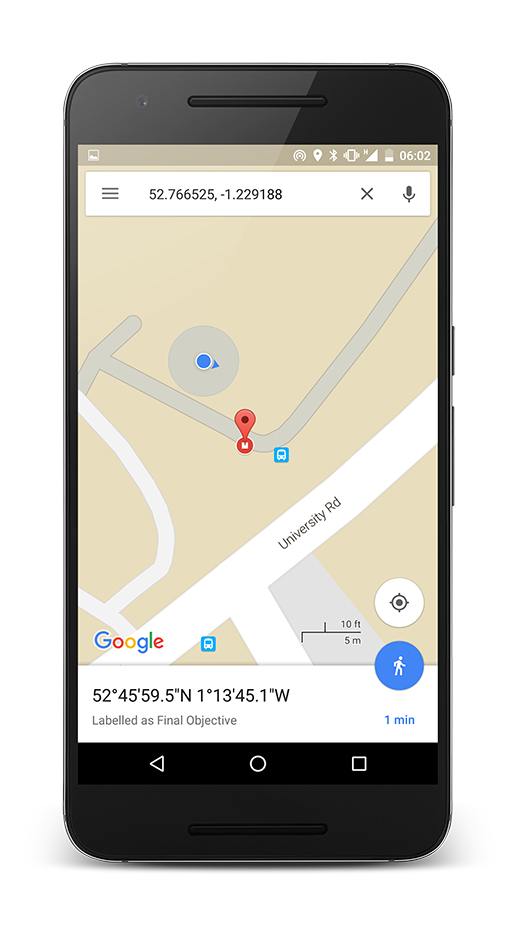
\includegraphics[width=1.0\textwidth]{phone_map_view_1}
  \caption{}
\endminipage
\end{figure}

\begin{figure}[!htb]
\minipage{0.32\textwidth}
  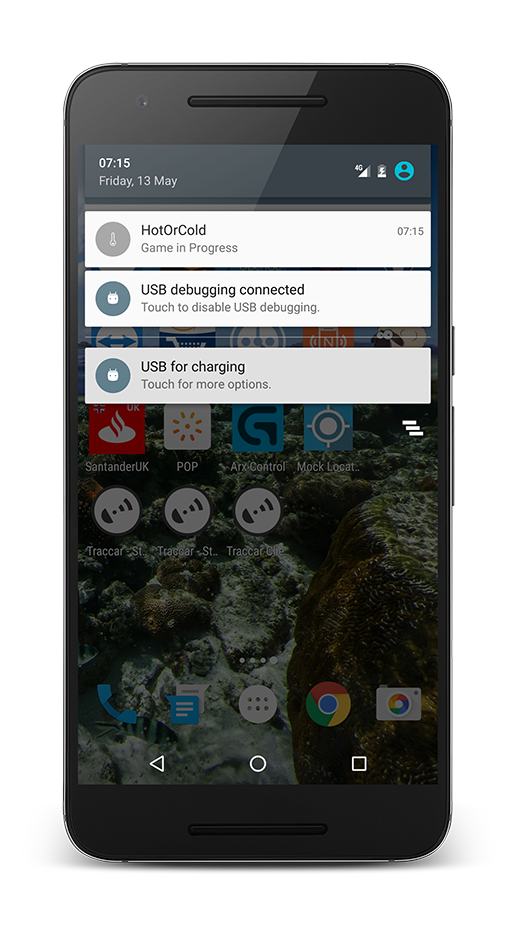
\includegraphics[width=1.0\textwidth]{phone_notification_1}
  \caption{}
\endminipage\hfill
\minipage{0.32\textwidth}
  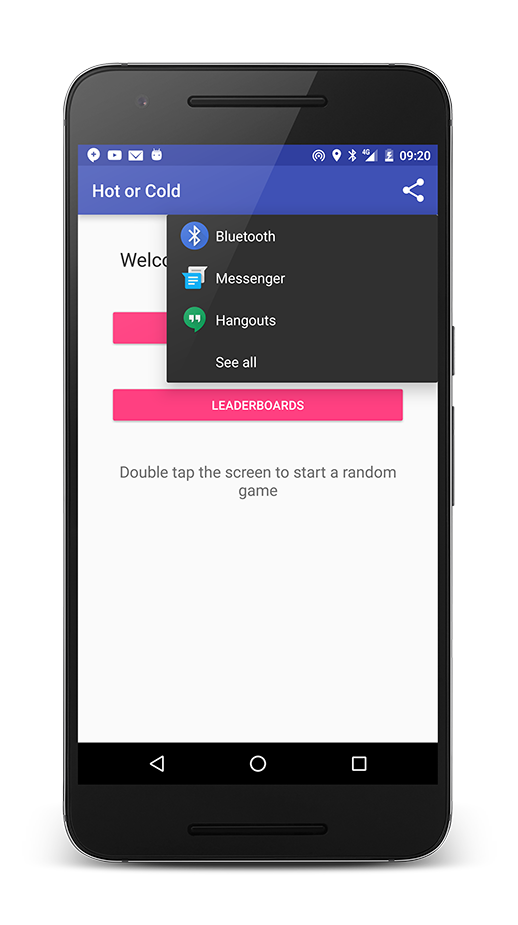
\includegraphics[width=1.0\textwidth]{phone_shareprovider_1}
  \caption{}
\endminipage\hfill
\minipage{0.32\textwidth}%
  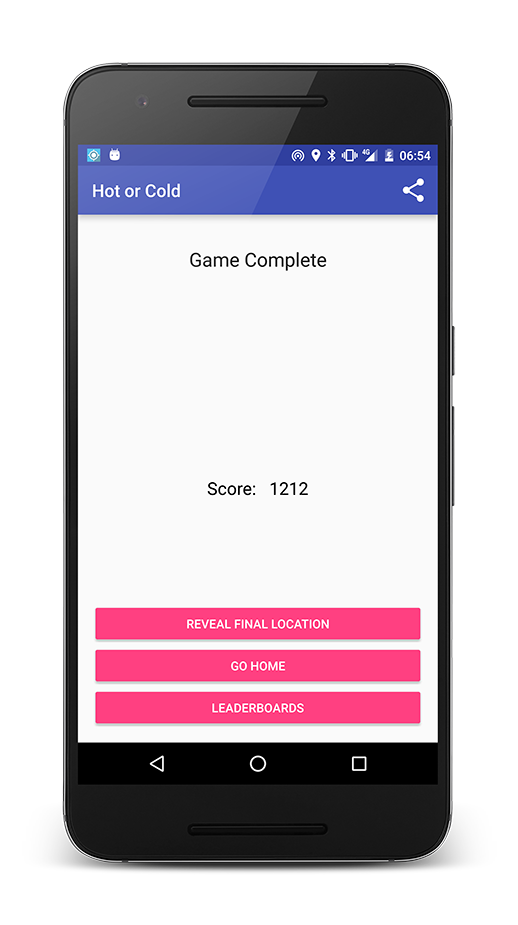
\includegraphics[width=1.0\textwidth]{phone_score_3}
  \caption{}
\endminipage
\end{figure}

\begin{figure}[!htb]
\minipage{0.32\textwidth}
  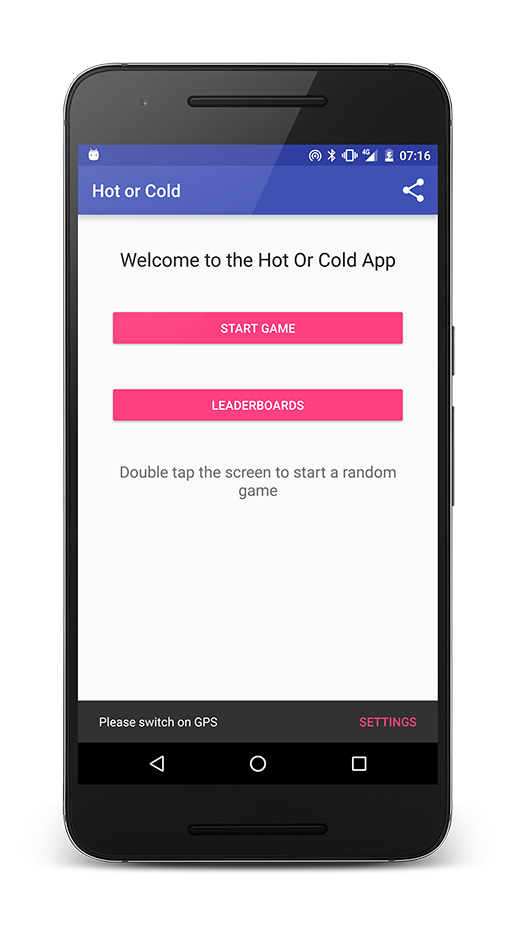
\includegraphics[width=1.0\textwidth]{phone_snackbar_1}
  \caption{}
\endminipage\hfill
\minipage{0.32\textwidth}
  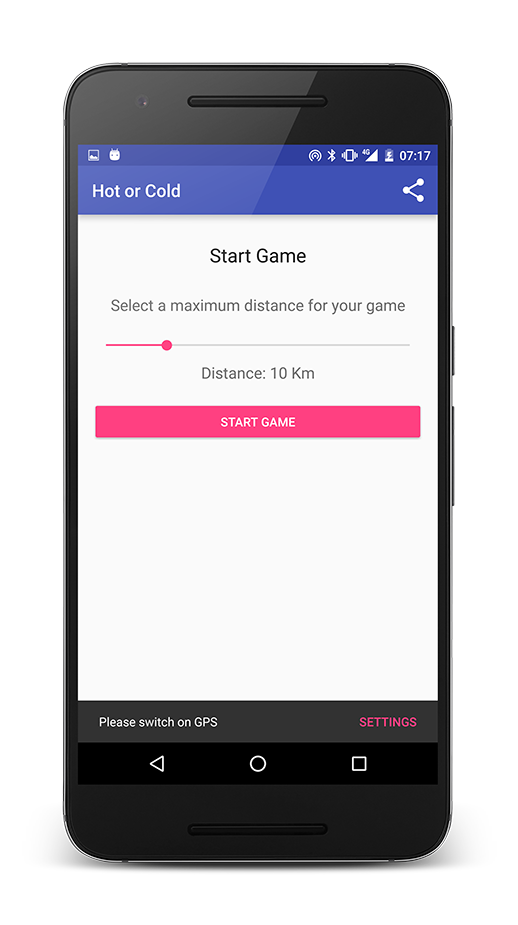
\includegraphics[width=1.0\textwidth]{phone_startgame_1}
  \caption{}
\endminipage\hfill
\minipage{0.32\textwidth}%
  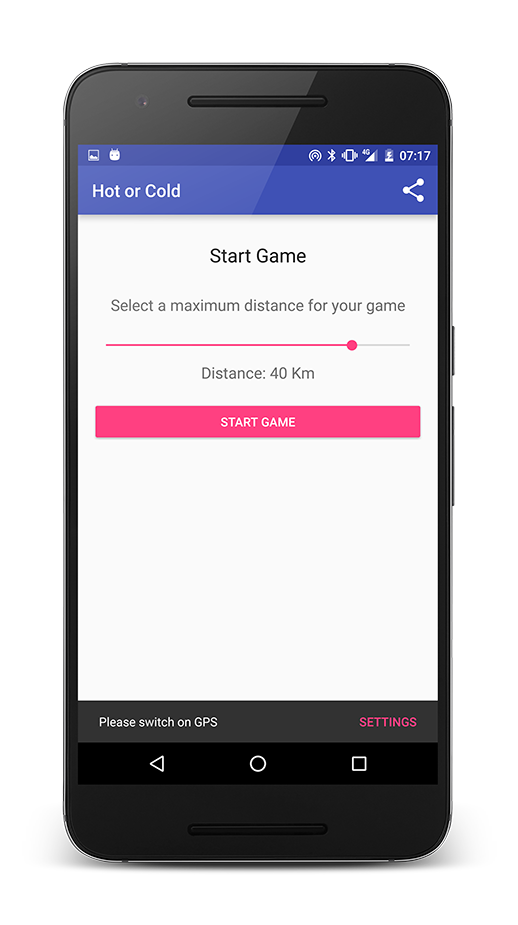
\includegraphics[width=1.0\textwidth]{phone_startgame_2}
  \caption{}
\endminipage
\end{figure}

\begin{figure}[!htb]
\minipage{1.0\textwidth}%
\begin{center}
  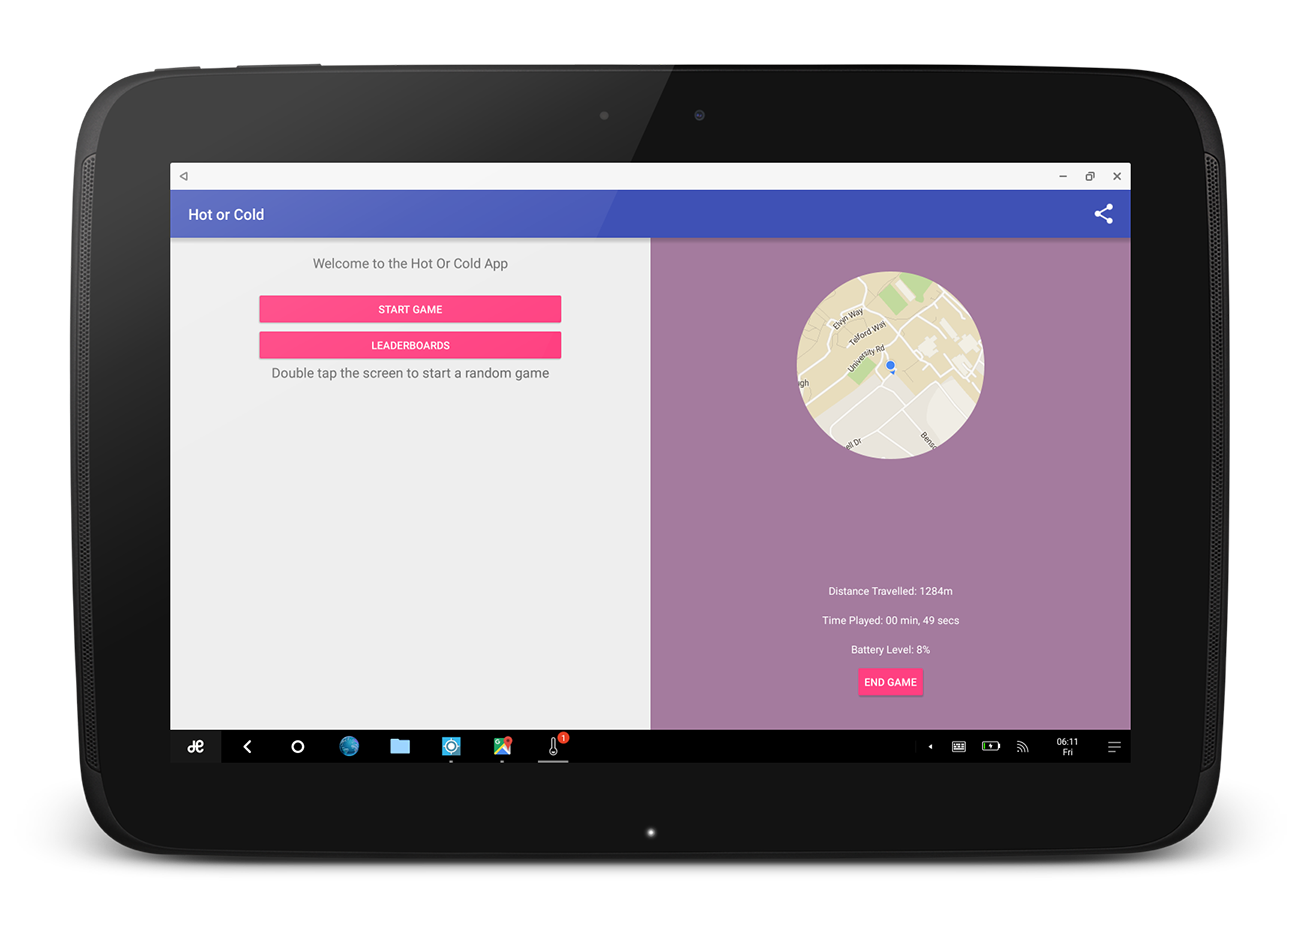
\includegraphics[width=0.9\textwidth]{tablet_game_1}
  \caption{}
\end{center}
\endminipage
\end{figure}

\begin{figure}[!htb]
\minipage{1.0\textwidth}%
\begin{center}
  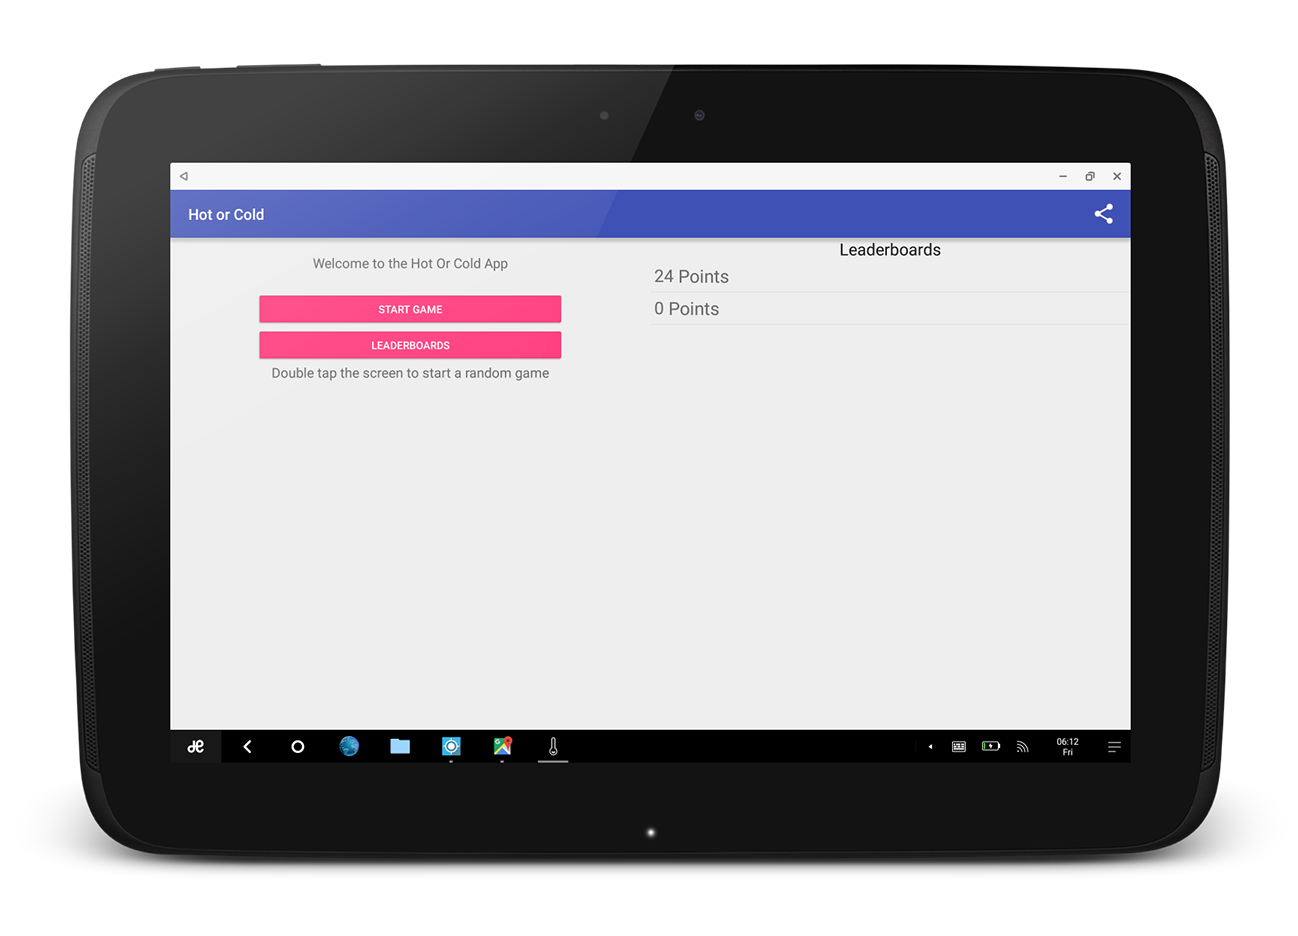
\includegraphics[width=0.9\textwidth]{tablet_leaderboard_1}
  \caption{}
\end{center}
\endminipage
\end{figure}

\begin{figure}[!htb]
\minipage{1.0\textwidth}%
\begin{center}
  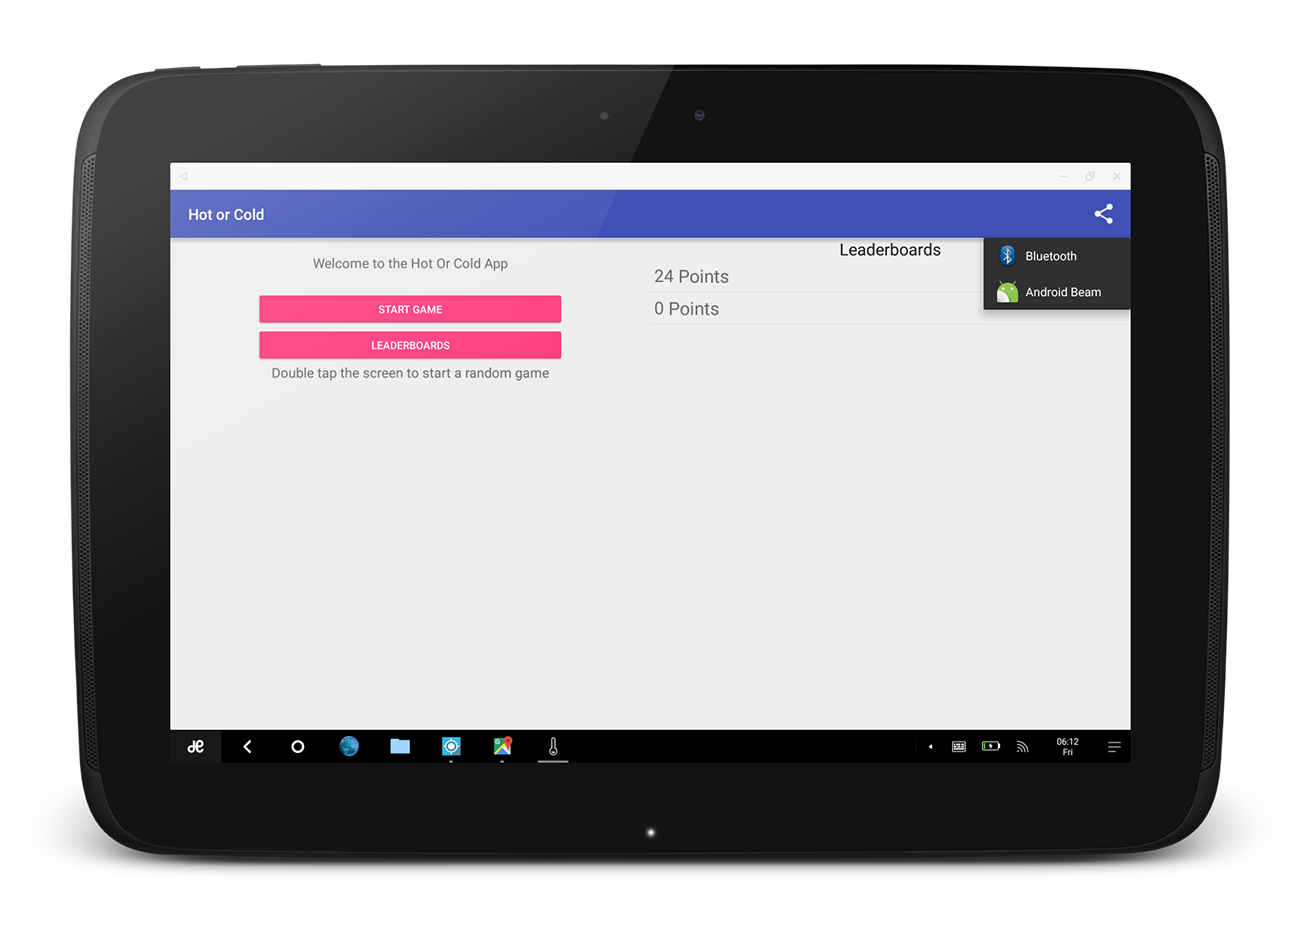
\includegraphics[width=0.9\textwidth]{tablet_share_1}
  \caption{}
\end{center}
\endminipage
\end{figure}

\begin{figure}[!htb]
\minipage{1.0\textwidth}%
\begin{center}
  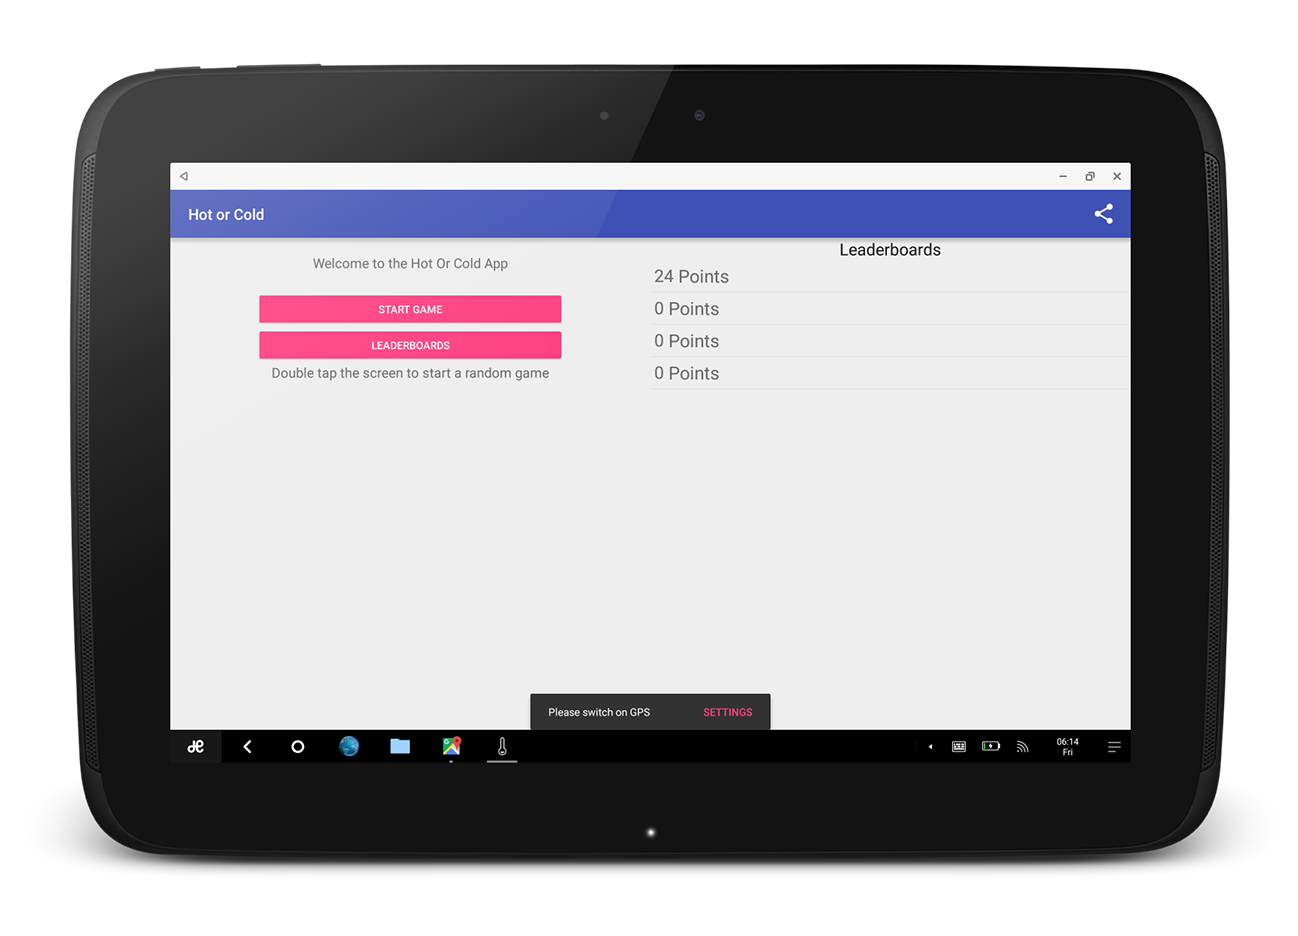
\includegraphics[width=0.9\textwidth]{tablet_snackbar_1}
  \caption{}
\end{center}
\endminipage
\end{figure}

\begin{figure}[!htb]
\minipage{1.0\textwidth}%
\begin{center}
  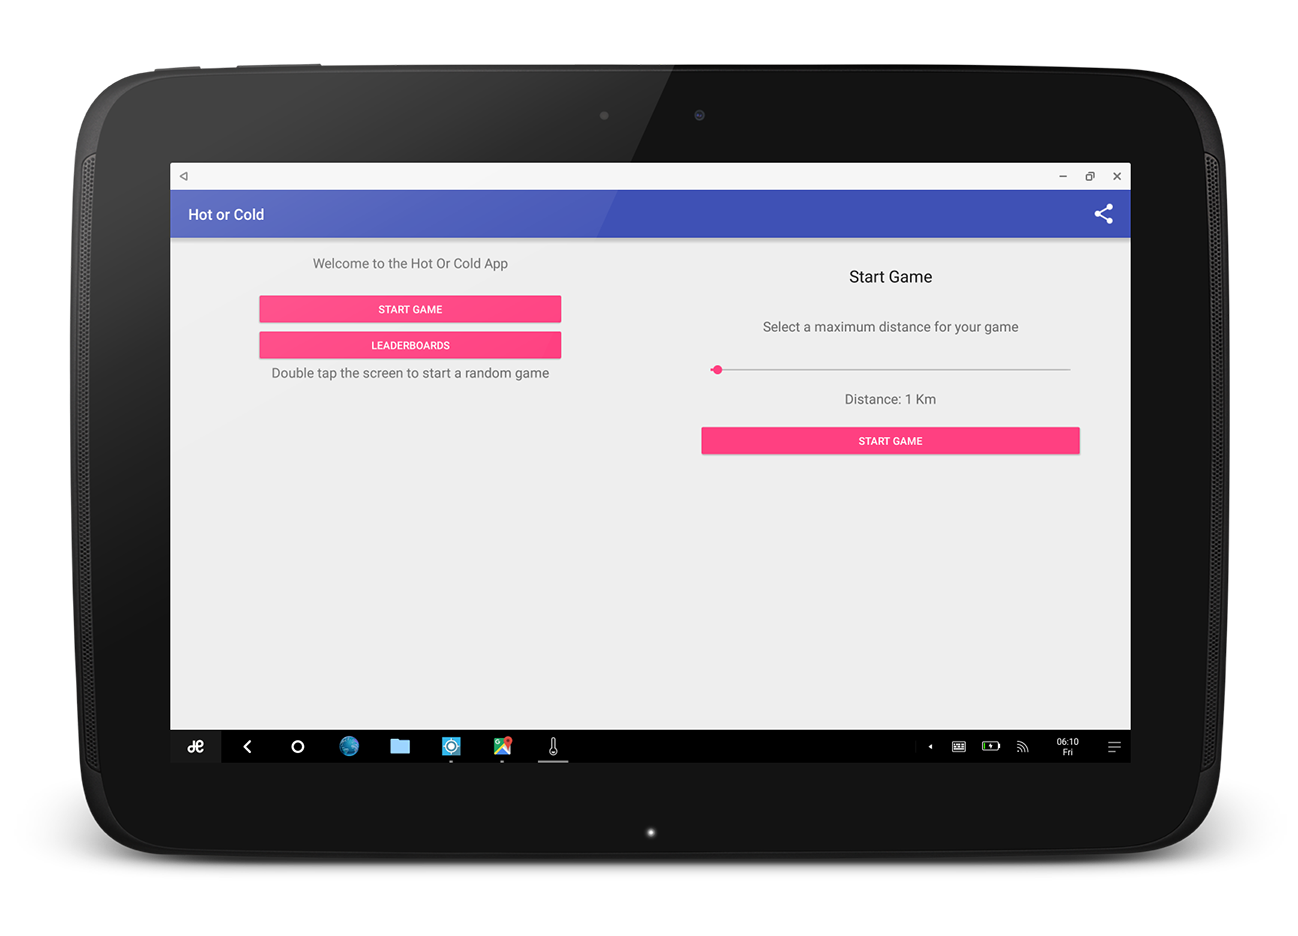
\includegraphics[width=0.9\textwidth]{tablet_startgame_1}
  \caption{}
\end{center}
\endminipage
\end{figure}

\begin{figure}[!htb]
\minipage{1.0\textwidth}%
\begin{center}
  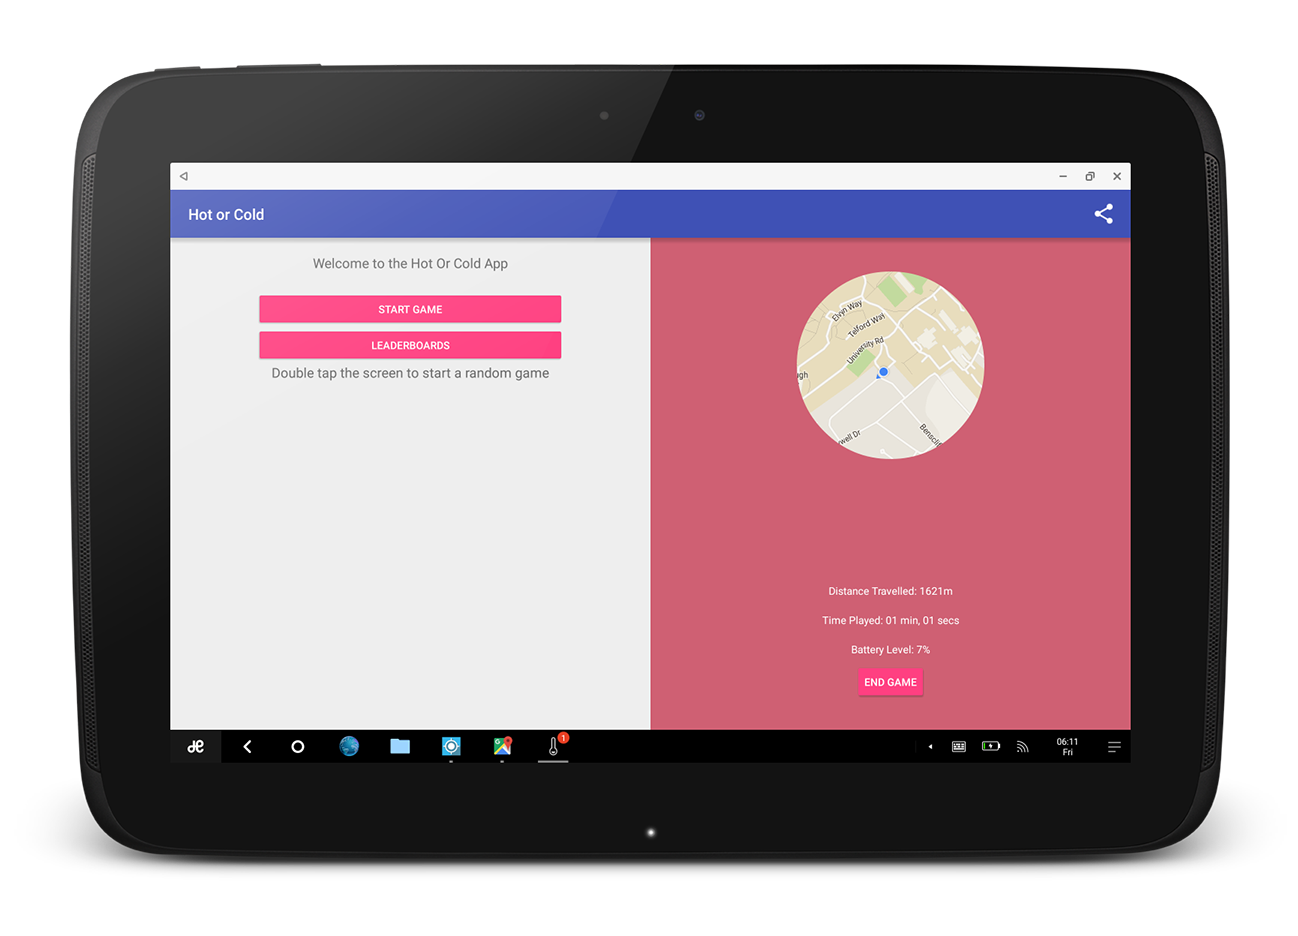
\includegraphics[width=0.9\textwidth]{tablet_startgame_2}
  \caption{}
\end{center}
\endminipage
\end{figure}

\end{document}